\documentclass[11pt,a4paper]{article}
\usepackage[utf8]{inputenc}
\usepackage[margin=1in]{geometry}
\usepackage{graphicx}
\usepackage{booktabs}
\usepackage{amsmath}
\usepackage{hyperref}
\usepackage{xcolor}
\usepackage{microtype}
\usepackage{float}
\usepackage{caption}
\usepackage{subcaption}

% Design/Formatting Customization
\definecolor{clinicalblue}{HTML}{1A5276}
\hypersetup{
    colorlinks=true,
    linkcolor=clinicalblue,
    filecolor=clinicalblue,      
    urlcolor=clinicalblue,
    citecolor=clinicalblue,
}
\usepackage{titlesec}
\titleformat{\section}
  {\normalfont\Large\bfseries\color{clinicalblue}}{\thesection}{1em}{}
\titleformat{\subsection}
  {\normalfont\large\bfseries\color{clinicalblue}}{\thesubsection}{1em}{}

\title{
    \vspace{-2cm}
    \textbf{\color{clinicalblue}Technical Report: Clinical Text Codification}\\
    \large{ICD-10 First-Character Chapter Classification NLP Challenge}
}
\author{\textbf{NLP Pipeline Team} \\ ASHO \& UAB Clinical Codification Project}
\date{\today}

\begin{document}

\maketitle

\begin{abstract}
Automating clinical codification is a critical task in healthcare administration, traditionally requiring manual translation of free-text clinical literals into structured codes. This report presents an end-to-end evaluation of a deep learning approach for predicting the first alphanumeric character of ICD-10 codes from short medical text literals in Spanish. We describe the exploratory data analysis of 13,700 samples, detail the construction of a TF-IDF and Logistic Regression baseline, and compare it against a deep learning architecture using a pre-trained clinical Spanish transformer (\texttt{roberta-base-biomedical-clinical-es}). The deep learning model achieves an accuracy of \textbf{57.01\%} and a Macro-$F_1$ score of \textbf{49.42\%}, representing absolute improvements of \textbf{+4.02\%} and \textbf{+4.93\%} over the baseline, respectively. Finally, we conduct a qualitative error analysis to characterize failure modes, including semantic overlaps, looking-glass character confusions, and dataset annotation noise.
\end{abstract}

\section{Introduction}
Clinical codification involves mapping free-text medical records (diagnoses, symptoms, and procedures) to standardized alphanumeric codes defined by the International Classification of Diseases, 10th Revision (ICD-10). In this challenge, the goal is scoped to predicting the first alphanumeric character of the target ICD-10 code based on a short clinical literal (e.g., \textit{``golpe contra muro''}, \textit{``itu pARTO''}). The first character indicates the broad medical category or chapter:
\begin{itemize}
    \item \textbf{Letters (A--Z):} Diagnosis chapters (e.g., \texttt{A} and \texttt{B} for infectious diseases, \texttt{C} for malignant neoplasms, \texttt{Z} for factors influencing health status).
    \item \textbf{Numbers (0--9):} Medical, surgical, and obstetrical procedure chapters.
\end{itemize}
The prediction task is structured as a 36-class single-label classification problem. The data is split into an 80\% training set and a 20\% validation set using a stratified split to preserve class proportions.

\section{Exploratory Data Analysis (EDA)}
We performed exploratory data analysis on the dataset using the script \texttt{eda\_analysis.py}. 

\subsection{Basic Corpus Statistics}
The dataset contains a total of \textbf{13,700 clinical text literals} spanning all 36 possible categories. Standard text length analysis shows that the literals are very short:
\begin{itemize}
    \item \textbf{Character Length:} Mean of $16.9$ characters (standard deviation $\sigma = 10.3$).
    \item \textbf{Word Count:} Mean of $2.2$ words (standard deviation $\sigma = 1.4$), with a median of $2.0$ words, and a maximum length of $18.0$ words.
\end{itemize}

\subsection{Severe Class Imbalance}
The dataset is characterized by an extreme class imbalance, which presents a significant challenge for model training and evaluation. The class counts range from a maximum of 1,715 samples to a minimum of 7 samples, yielding an \textbf{imbalance ratio of 245.0x}.
\begin{itemize}
    \item \textbf{Top 3 Most Frequent Categories:}
    \begin{enumerate}
        \item \texttt{Z} (Health status / Services): 1,715 samples (12.52\% of the corpus)
        \item \texttt{O} (Pregnancy / Childbirth): 1,507 samples (11.00\%)
        \item \texttt{0} (Procedures - Medical/Surgical): 1,141 samples (8.33\%)
    \end{enumerate}
    \item \textbf{Least Frequent Categories (Support $\le 20$):}
    \begin{itemize}
        \item \texttt{W} (External causes - falls): 7 samples (0.05\%)
        \item \texttt{X} (External causes - other): 11 samples (0.08\%)
        \item \texttt{A} (Infectious diseases - bacteria/viruses): 18 samples (0.13\%)
        \item \texttt{Y} (External causes - surgery/medical): 36 samples (0.26\%)
        \item \texttt{U} (Special purposes): 21 samples (0.15\%)
    \end{itemize}
\end{itemize}
The class frequency and text length distributions are visualized in Figure~\ref{fig:class_dist} and Figure~\ref{fig:length_dist}, respectively.

\begin{figure}[H]
    \centering
    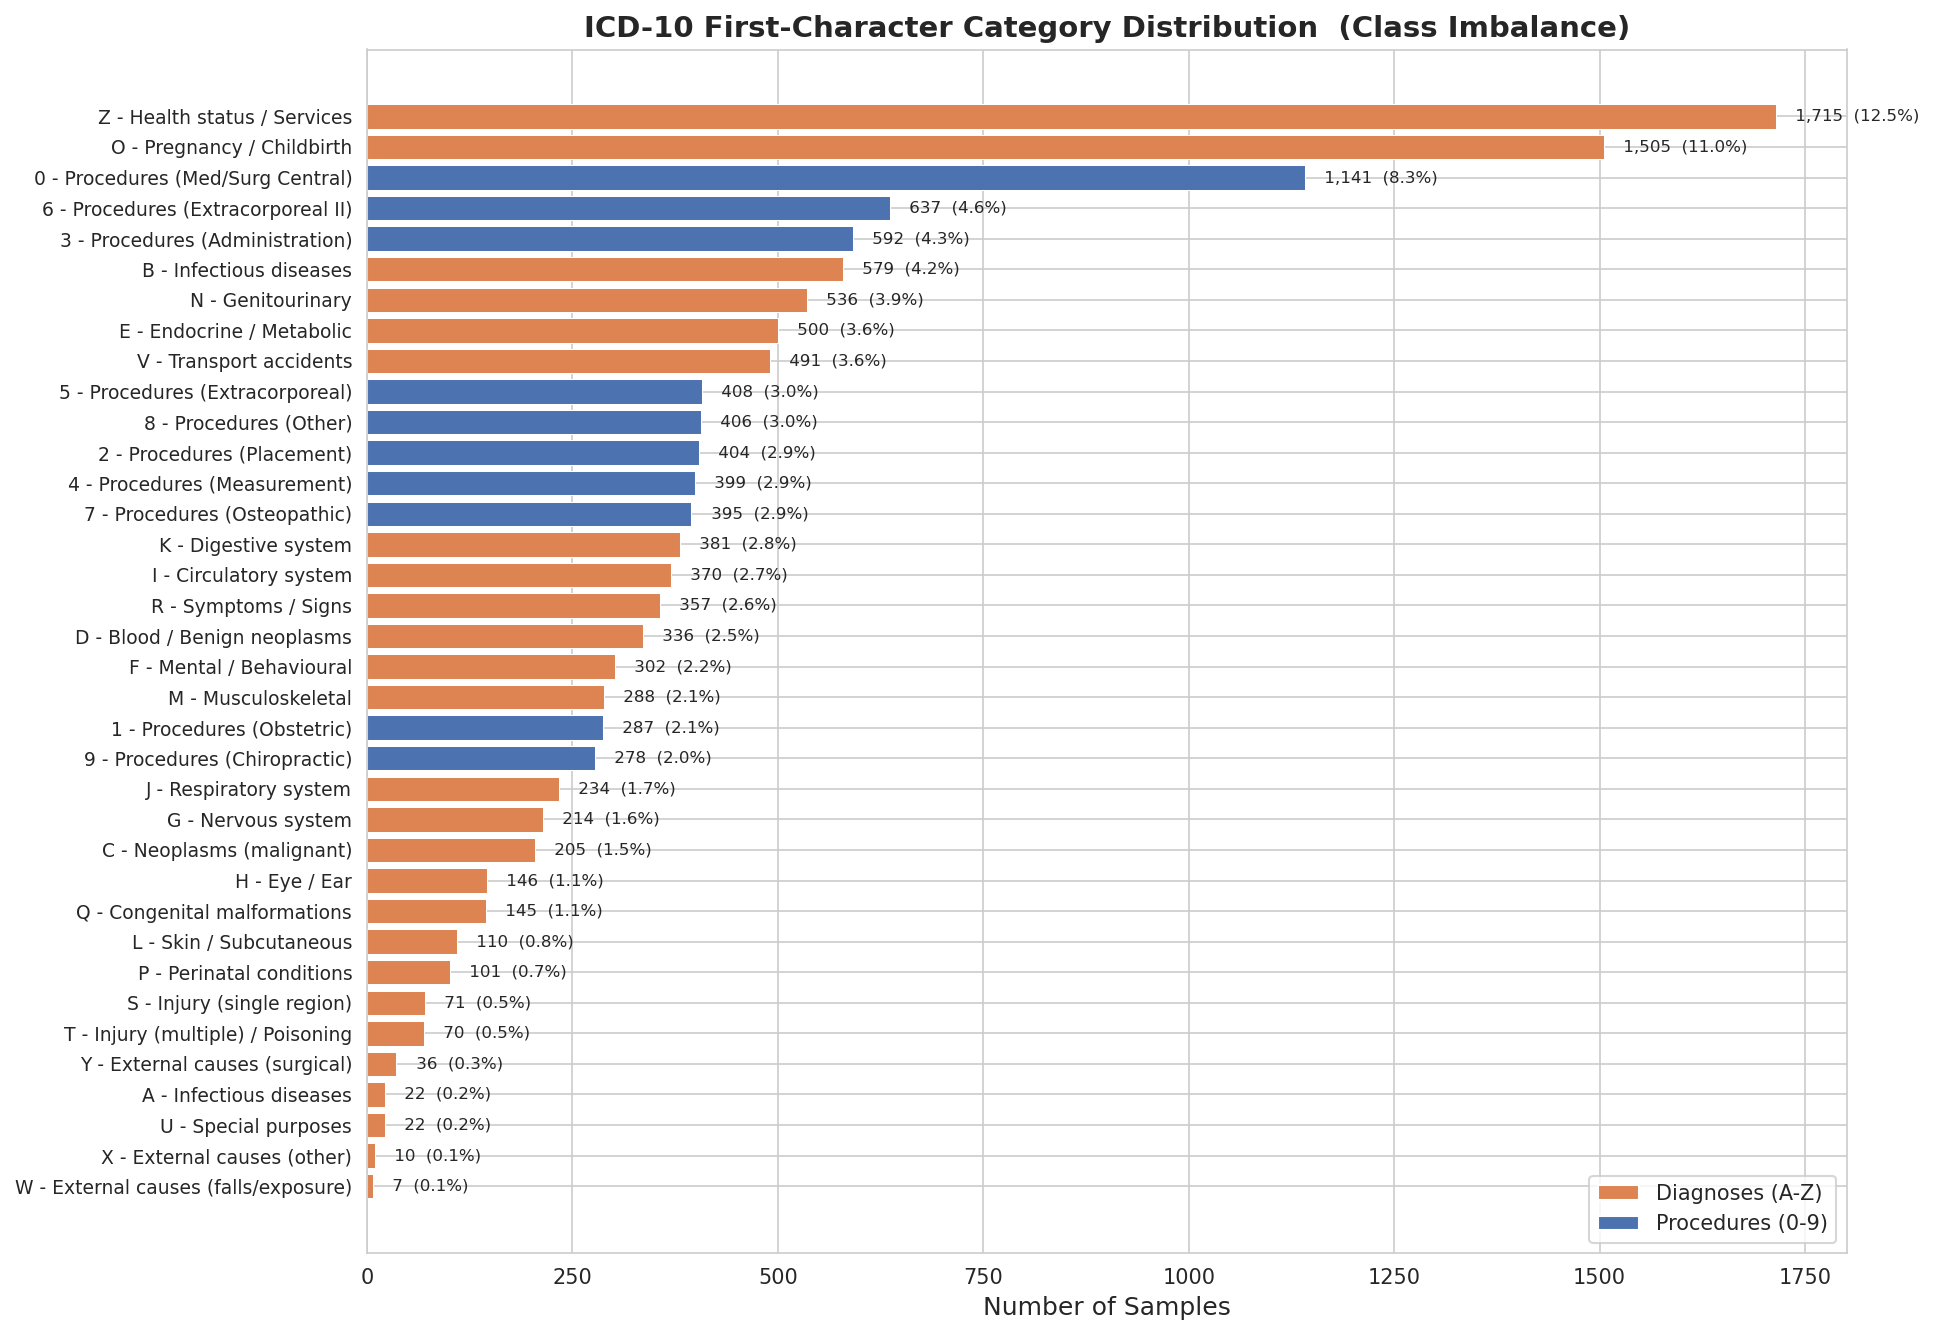
\includegraphics[width=0.9\textwidth]{eda_class_distribution.png}
    \caption{Class Frequencies across Chapters}
    \label{fig:class_dist}
\end{figure}

\begin{figure}[H]
    \centering
    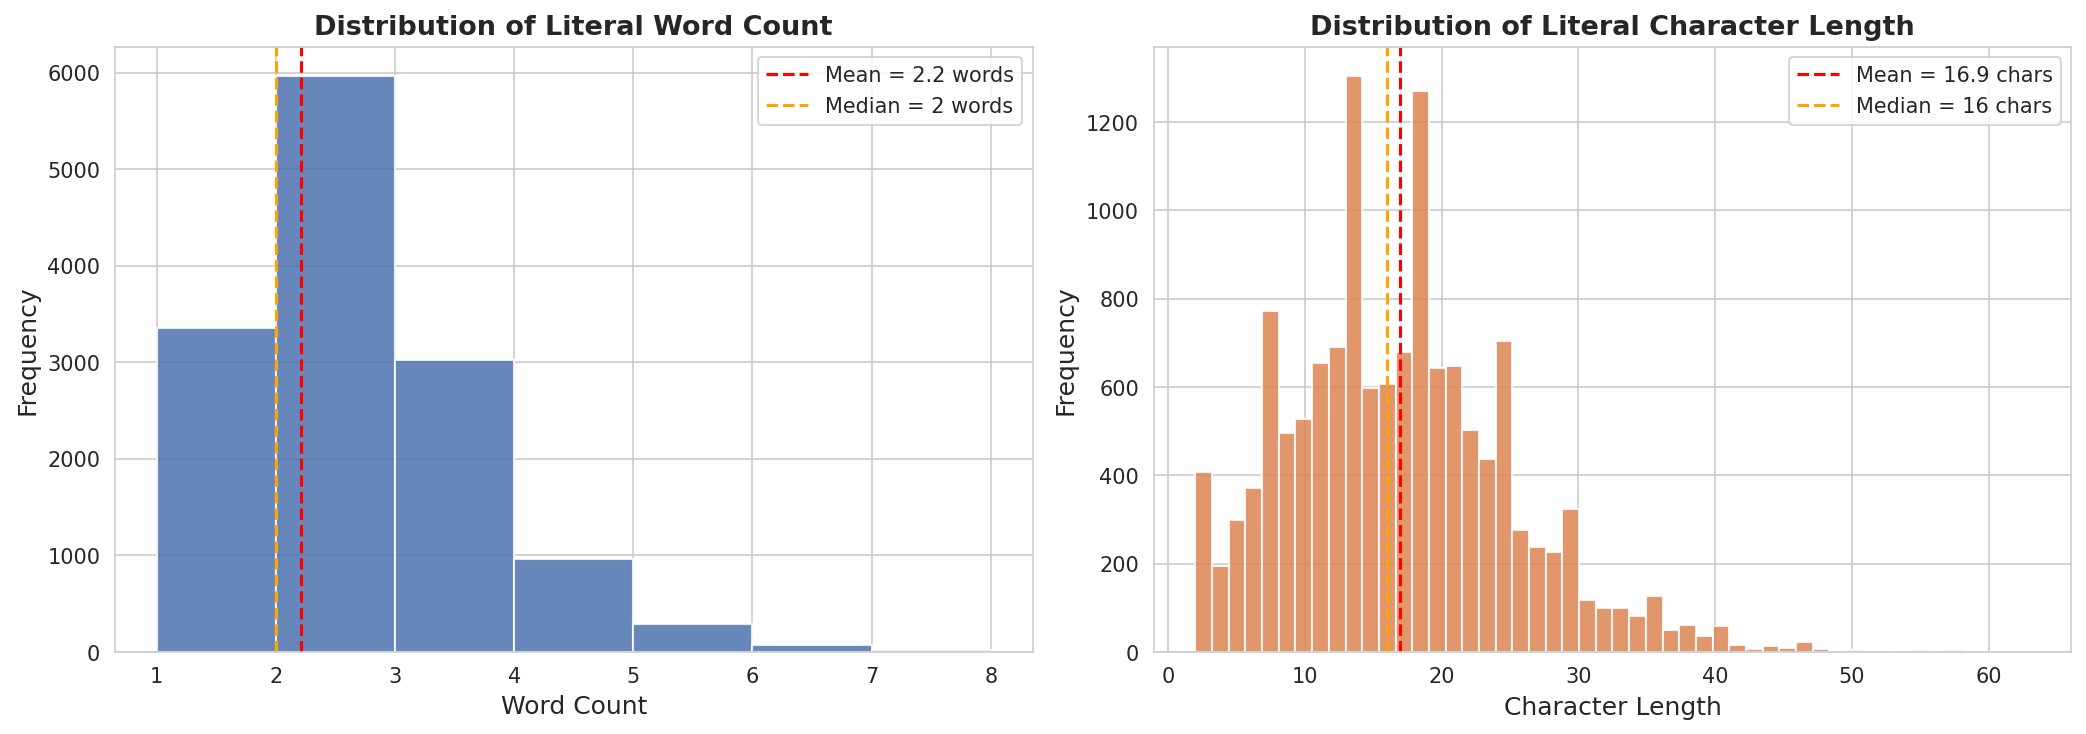
\includegraphics[width=0.9\textwidth]{eda_text_length_distribution.png}
    \caption{Distribution of Text Lengths}
    \label{fig:length_dist}
\end{figure}

\section{Methodology}
To establish performance bounds, we evaluated two distinct architectural paradigms. Both were trained and tested on the identical 80/20 stratified split (using random seed 42) to ensure a rigorous comparison.

\subsection{Baseline Pipeline (TF-IDF + Logistic Regression)}
We built a baseline system in Scikit-Learn utilizing a hybrid feature extraction pipeline:
\begin{enumerate}
    \item \textbf{Character $n$-gram Vectorizer:} Extracts character $n$-grams ranging from 3 to 5 characters (maximum features: 100,000). This captures clinical root words, suffixes, prefixes, and minor typos.
    \item \textbf{Word $n$-gram Vectorizer:} Extracts unigrams and bigrams (maximum features: 50,000) to represent whole terms.
\end{enumerate}
These vectorizer outputs are joined via a \texttt{FeatureUnion} and passed to a multinomial Logistic Regression classifier with LBFGS optimization and default regularization ($C=1.0$).

\subsection{Deep Learning Pipeline (RoBERTa + Attention Pooling)}
The neural network model is built on top of the pre-trained clinical language model \texttt{PlanTL-GOB-ES/roberta-base-biomedical-clinical-es}, which has been pre-trained on Spanish clinical texts. To capture textual features effectively, we discarded the simple class-token representation and implemented:
\begin{itemize}
    \item \textbf{Attention Pooling:} Calculates a weighted sum over the token embeddings using a learnable attention mechanism, allowing the model to focus on key clinical terms.
    \item \textbf{Multi-Sample Dropout:} We used 5 parallel dropout layers ($p=0.1$) before the final classification head to reduce overfitting and speed up convergence.
    \item \textbf{Loss & Optimization:} The model was trained using Cross-Entropy Loss with the AdamW optimizer, a cosine learning rate scheduler with warmup, and gradient accumulation.
\end{itemize}

\section{Quantitative Results}
The evaluation on the 2,740 validation samples shows that the deep learning model outperforms the TF-IDF baseline across all core metrics. The comparison is summarized in Table~\ref{tab:comparison}.

\begin{table}[H]
\centering
\caption{Model Evaluation and Comparison (Validation Set)}
\label{tab:comparison}
\begin{tabular}{lccc}
\toprule
\textbf{Metric} & \textbf{TF-IDF + Logistic Regression} & \textbf{RoBERTa + Attention Pooling} & \textbf{Delta ($\Delta$)} \\
\midrule
\textbf{Accuracy} & 52.99\% & \textbf{57.01\%} & \textbf{+4.02\%} \\
\textbf{Macro-$F_1$} & 44.49\% & \textbf{49.42\%} & \textbf{+4.93\%} \\
\textbf{Weighted-$F_1$} & 51.04\% & \textbf{55.07\%} & \textbf{+4.03\%} \\
\bottomrule
\end{tabular}
\end{table}

The absolute improvement in Macro-$F_1$ (+4.93\%) is particularly notable because it indicates that the deep learning model handles class imbalance more robustly, achieving better recall and precision on the tail categories compared to the baseline.

\section{Detailed Error Analysis}
An error analysis was performed on the validation set predictions to characterize the deep learning model's failure modes. Out of 2,740 validation samples, the deep learning model committed \textbf{1,178 errors} (a 43.0\% error rate). The confusion heatmap is visualized in Figure~\ref{fig:cm_heatmap}, and the top 15 most frequent error pairs are plotted in Figure~\ref{fig:top_errors}.

\begin{figure}[H]
    \centering
    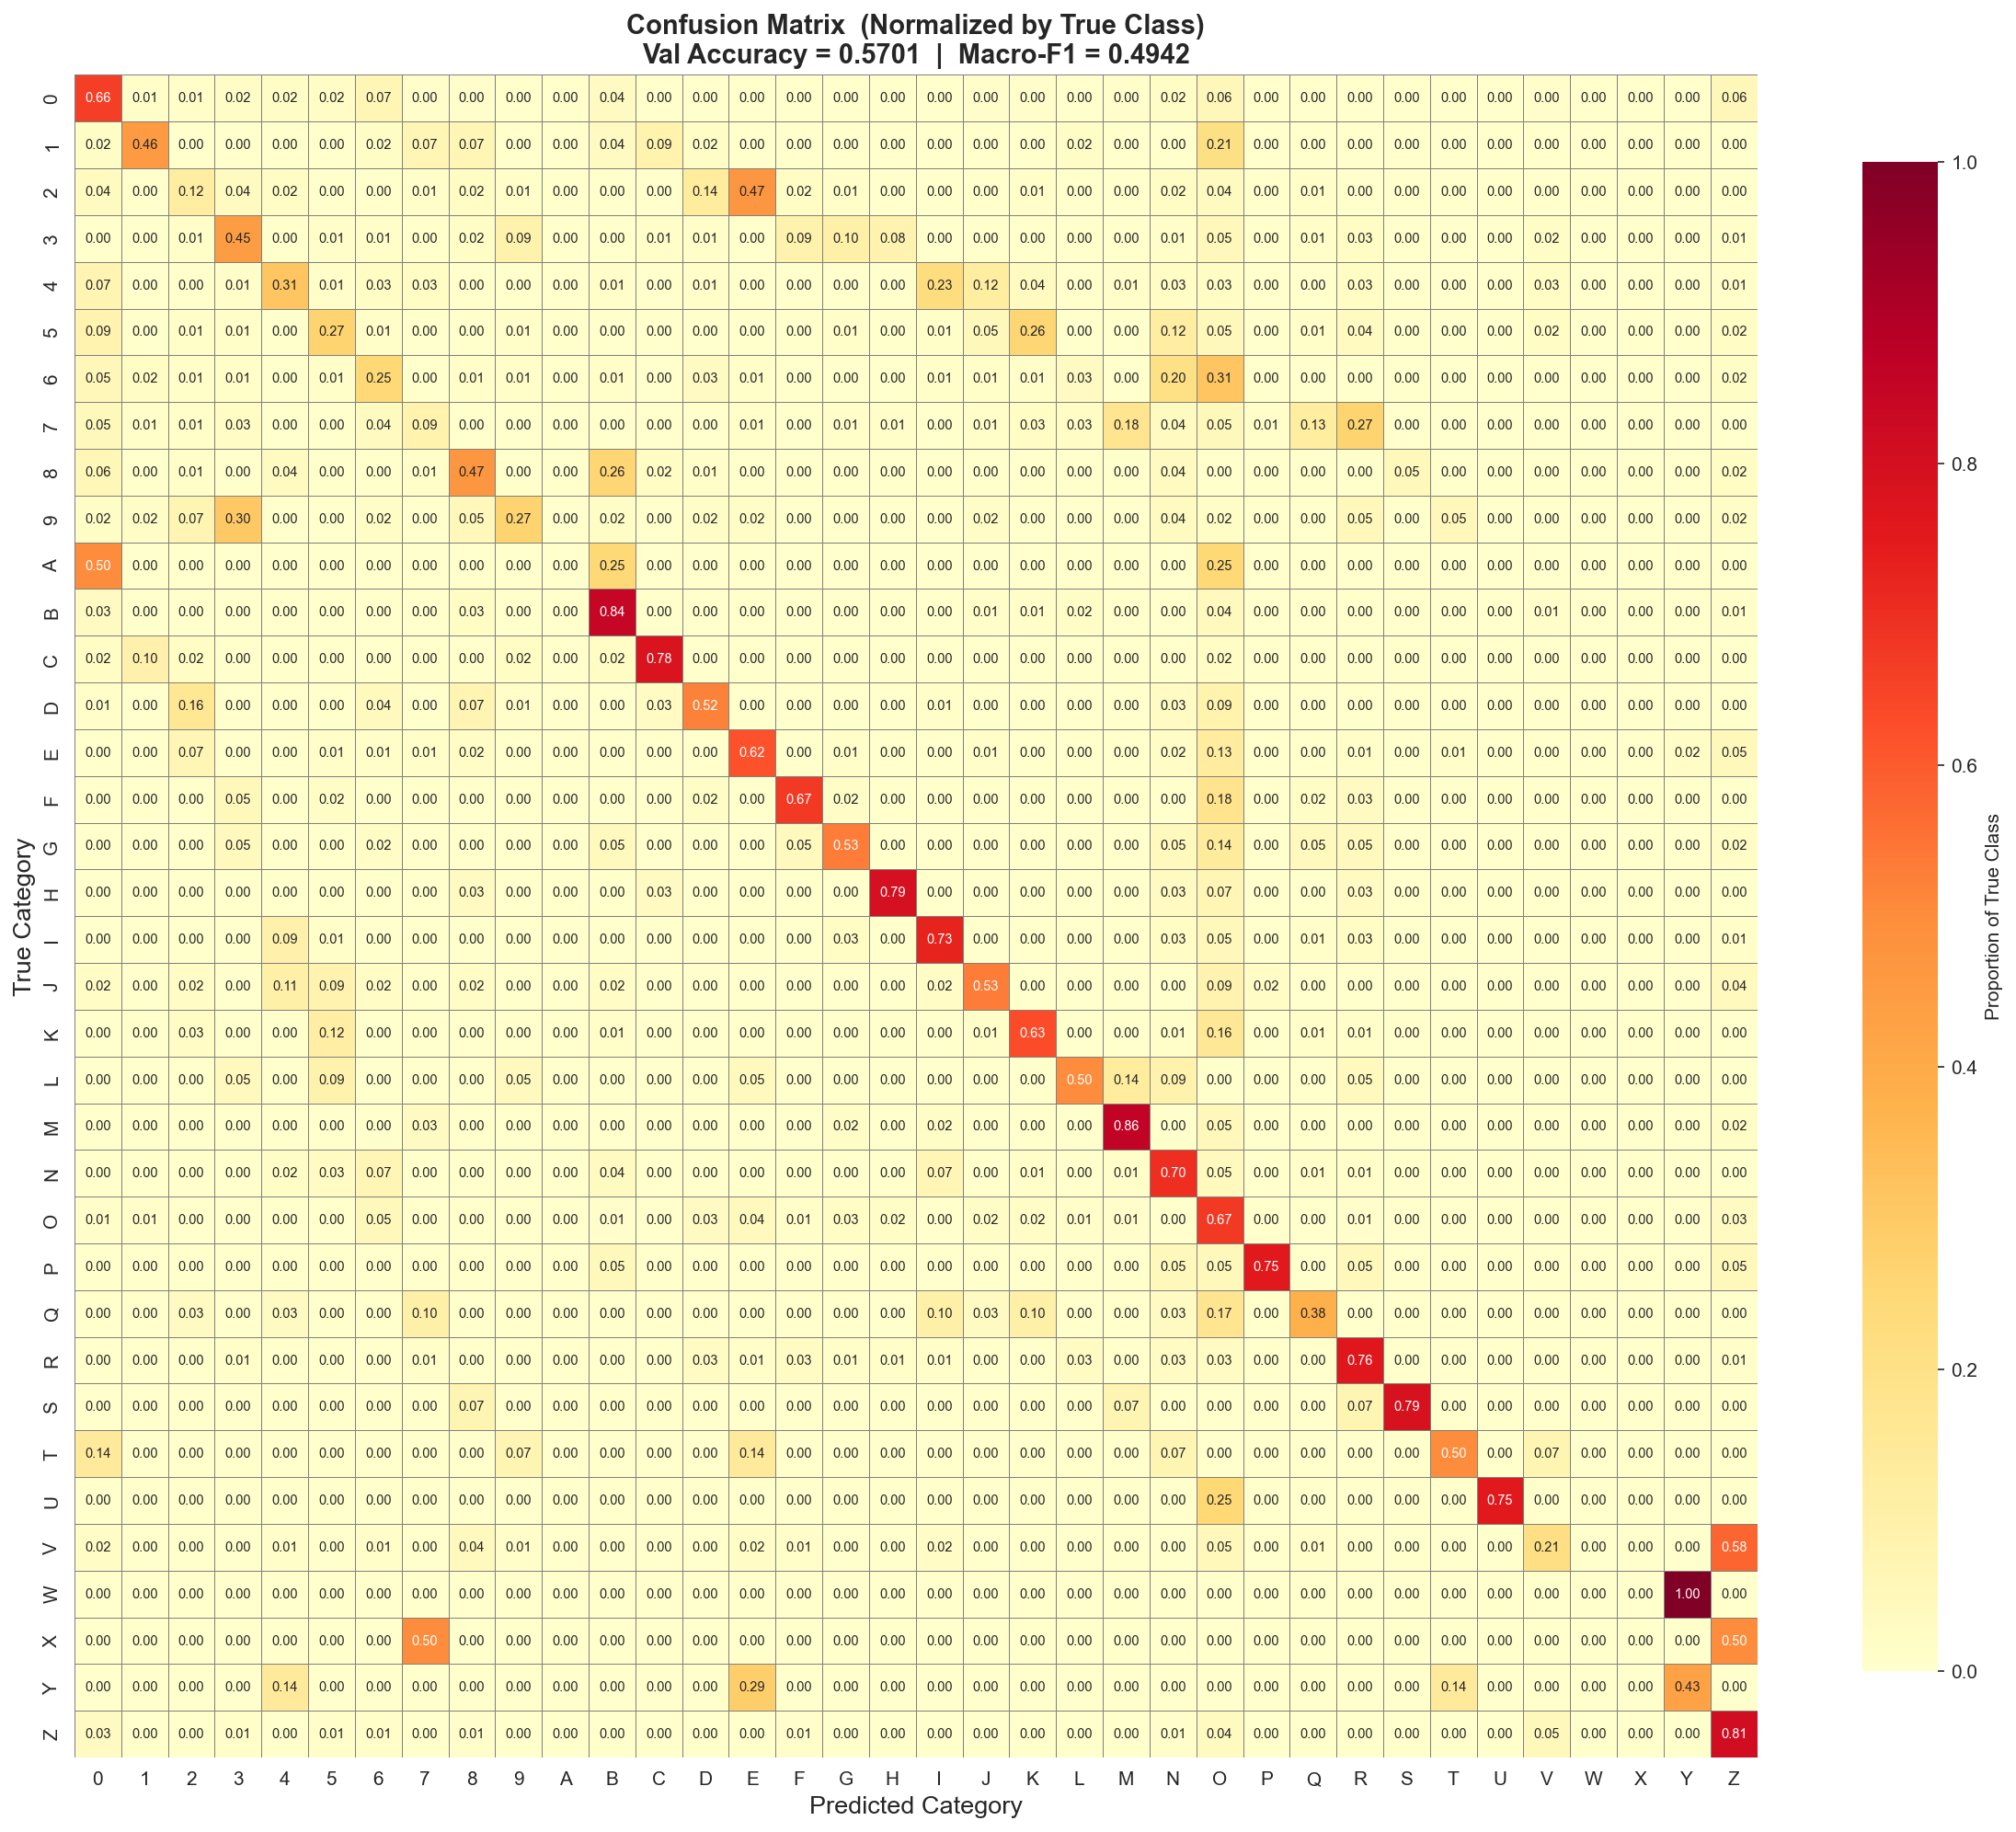
\includegraphics[width=0.85\textwidth]{error_confusion_matrix.png}
    \caption{Normalized Confusion Heatmap}
    \label{fig:cm_heatmap}
\end{figure}

\begin{figure}[H]
    \centering
    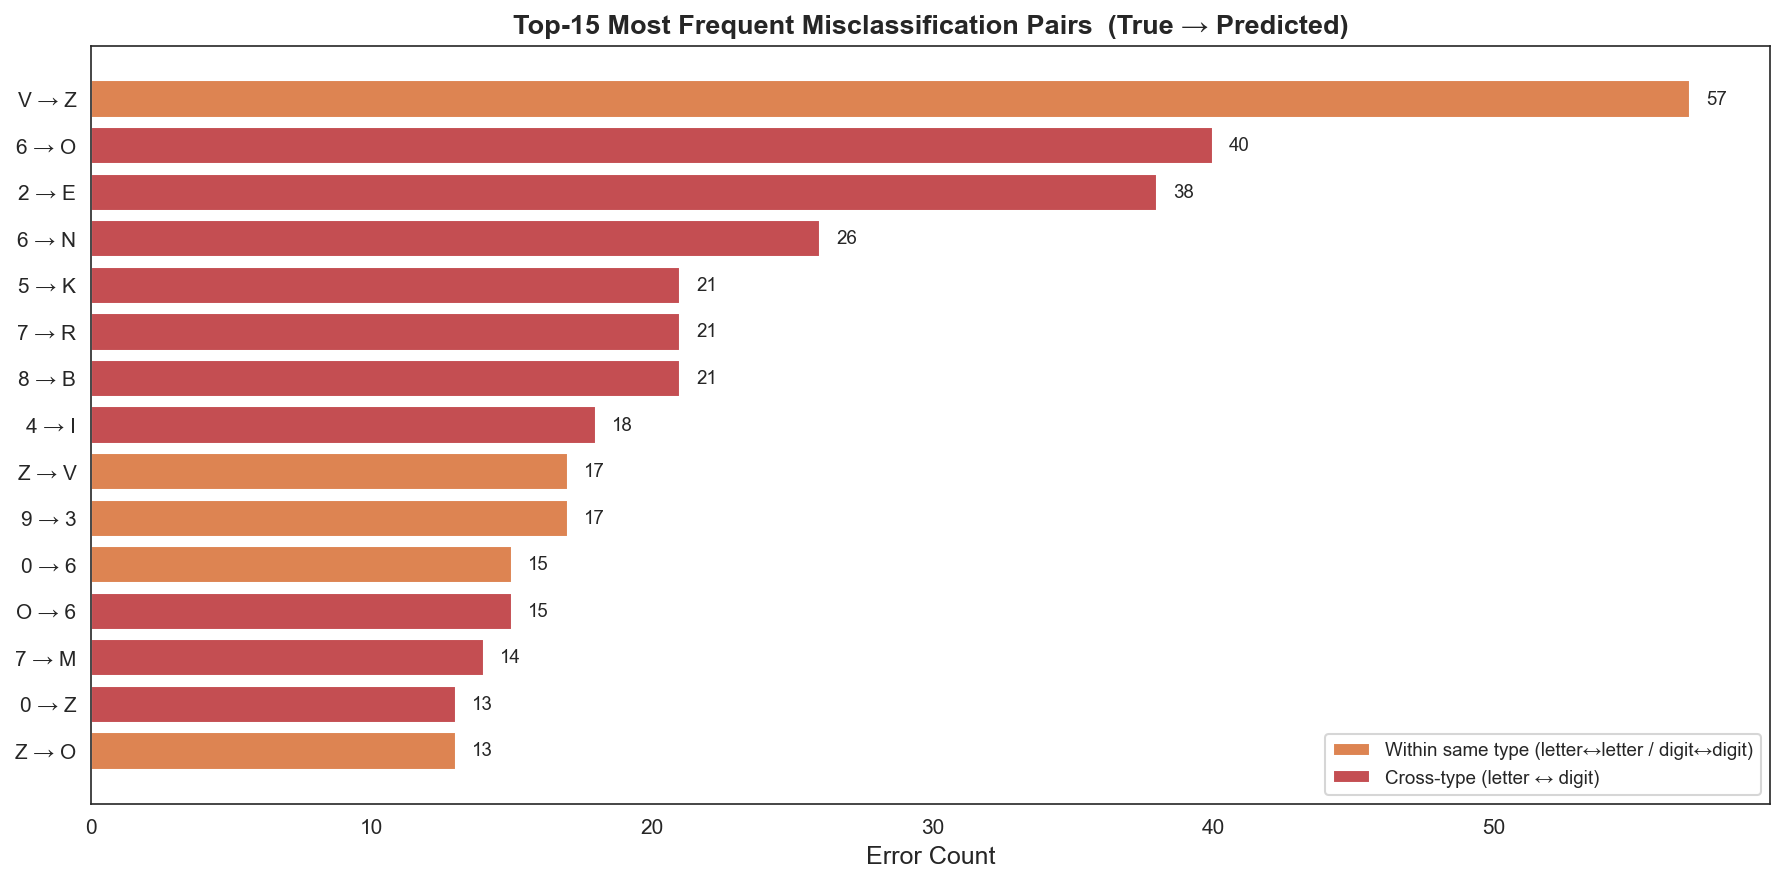
\includegraphics[width=0.9\textwidth]{error_top_confusions.png}
    \caption{Top 15 Misclassification Pairs}
    \label{fig:top_errors}
\end{figure}

\subsection{Analysis of Specific Error Modes}

\subsubsection{Neoplasm Subtype Confusion (Chapter C vs. D)}
We investigated the confusion between Malignant Neoplasms (\texttt{C}) and Blood/Benign Neoplasms (\texttt{D}). Surprisingly, the model displays exceptional granularity, making only \textbf{2 errors} total between these chapters on the validation set. 
\begin{itemize}
    \item \textit{Literal:} ``Adenocarcinoma in situ endocervical'' $\rightarrow$ True: \texttt{D}, Pred: \texttt{C} (Confidence: 0.600)
    \item \textit{Literal:} ``tumor mucinoso borderline ovario izq'' $\rightarrow$ True: \texttt{D}, Pred: \texttt{C} (Confidence: 0.629)
\end{itemize}
This indicates that the clinical BERT embedding space is well-attuned to the semantic difference between benign/borderline and malignant terms (such as ``in situ'' or ``borderline'').

\subsubsection{Letter and Digit Look-Alikes}
Due to the alphanumeric layout, we analyzed whether standard characters are confused with similar-looking digits:
\begin{itemize}
    \item \textbf{Letter \texttt{O} (Pregnancy) vs. Digit \texttt{0} (Procedures):} Only \textbf{4 errors} occurred. These are mostly related to injuries or childbirth complications that the model maps to procedure-based words (e.g., \textit{``Desgarro 1''} $\rightarrow$ True: \texttt{O}, Predicted: \texttt{0}, Confidence: 0.708).
    \item \textbf{Letter \texttt{Z} (Health Status) vs. Digit \texttt{0} (Procedures):} \textbf{12 errors}. This confusion stems from surgical history described as a current status (e.g., \textit{``Anexectomía izquierda''}, \textit{``Histerectomía''}, \textit{``By pass Aortobifemoral''}), where the model maps the surgical nouns to surgical procedures (\texttt{0}) rather than health-status codes (\texttt{Z}).
    \item \textbf{Digit \texttt{6} (Extracorporeal Procedures) vs. Letter \texttt{O} (Pregnancy):} This is a major confusion axis, representing \textbf{40 errors} where true \texttt{6} was predicted as \texttt{O}, and \texttt{15 errors} where true \texttt{O} was predicted as \texttt{6}. This is driven by obstetric monitoring procedures (e.g., Non-Stress Tests or labor tracking) occurring during birth (e.g., \textit{``itu pARTO''} $\rightarrow$ True: \texttt{6}, Predicted: \texttt{O}, Confidence: 0.809).
\end{itemize}

\subsubsection{Top Global Confusions}
The most frequent error pair in the entire validation set is \textbf{\texttt{V} (Transport accidents) predicted as \texttt{Z} (Health status / Services)} with 57 errors. 
This occurs because patients presenting with injuries or histories of accidents are often documented in ways that resemble routine checkups or follow-up consults, leading the model to predict the general clinic visit code (\texttt{Z}) instead of the external injury cause (\texttt{V}). An example includes:
\begin{itemize}
    \item \textit{Literal:} ``alergia Àcars'' (dust mite allergy) $\rightarrow$ True: \texttt{V} (likely a labeling anomaly), Predicted: \texttt{Z} (Confidence: 0.990)
\end{itemize}

\subsection{High-Confidence Errors}
There are 402 instances where the model predicted a category with $\ge 70\%$ confidence but was incorrect. A qualitative examination reveals that many of these errors are due to \textbf{annotation noise} or highly ambiguous literals in the dataset:
\begin{itemize}
    \item \textit{Literal:} ``Febre rn'' (Newborn fever) $\rightarrow$ True: \texttt{7} (Osteopathic Procedures - likely an administrative coding error), Predicted: \texttt{P} (Perinatal Conditions, Confidence: 0.991)
    \item \textit{Literal:} ``Cataratas bilateras'' (Bilateral cataracts) $\rightarrow$ True: \texttt{3} (Measurement/Administration), Predicted: \texttt{H} (Diseases of the Eye, Confidence: 0.980)
    \item \textit{Literal:} ``Hipoacusia bilateral'' (Bilateral hearing loss) $\rightarrow$ True: \texttt{3} (Measurement/Administration), Predicted: \texttt{H} (Diseases of the Ear, Confidence: 0.975)
\end{itemize}
These cases indicate that the model's errors are often semantically logical, and that the ground-truth annotations in the clinical database contain systematic noise or specialized administrative guidelines that do not align with raw text semantics.

\section{Conclusion and Future Work}
This report outlines the successful implementation and evaluation of a clinical language model for Spanish ICD-10 chapter classification. By moving from a TF-IDF baseline to a pre-trained RoBERTa model with attention pooling, we achieved a \textbf{+4.02\% Accuracy} and \textbf{+4.93\% Macro-$F_1$} improvement.

Future iterations of the pipeline should focus on:
\begin{enumerate}
    \item \textbf{Imbalance Mitigation:} Applying loss-weighting techniques (e.g., Focal Loss or class-balanced weights) to improve performance on tail classes with under 20 training samples.
    \item \textbf{Data Cleaning:} Conducting manual review and filtering of high-confidence errors to correct systematic administrative misannotations (such as mapping cataracts to administrative codes rather than eye disorders).
    \item \textbf{Tokenization Adjustments:} Injecting character-level representations into the transformer embeddings to help resolve look-alike numeric vs. alphabetic ambiguities.
\end{enumerate}

\end{document}
